\documentclass[fleqn,10pt,lineno]{wlpeerj}\usepackage[]{graphicx}\usepackage[]{color}
%% maxwidth is the original width if it is less than linewidth
%% otherwise use linewidth (to make sure the graphics do not exceed the margin)
\makeatletter
\def\maxwidth{ %
  \ifdim\Gin@nat@width>\linewidth
    \linewidth
  \else
    \Gin@nat@width
  \fi
}
\makeatother

\definecolor{fgcolor}{rgb}{0.345, 0.345, 0.345}
\newcommand{\hlnum}[1]{\textcolor[rgb]{0.686,0.059,0.569}{#1}}%
\newcommand{\hlstr}[1]{\textcolor[rgb]{0.192,0.494,0.8}{#1}}%
\newcommand{\hlcom}[1]{\textcolor[rgb]{0.678,0.584,0.686}{\textit{#1}}}%
\newcommand{\hlopt}[1]{\textcolor[rgb]{0,0,0}{#1}}%
\newcommand{\hlstd}[1]{\textcolor[rgb]{0.345,0.345,0.345}{#1}}%
\newcommand{\hlkwa}[1]{\textcolor[rgb]{0.161,0.373,0.58}{\textbf{#1}}}%
\newcommand{\hlkwb}[1]{\textcolor[rgb]{0.69,0.353,0.396}{#1}}%
\newcommand{\hlkwc}[1]{\textcolor[rgb]{0.333,0.667,0.333}{#1}}%
\newcommand{\hlkwd}[1]{\textcolor[rgb]{0.737,0.353,0.396}{\textbf{#1}}}%
\let\hlipl\hlkwb

\usepackage{framed}
\makeatletter
\newenvironment{kframe}{%
 \def\at@end@of@kframe{}%
 \ifinner\ifhmode%
  \def\at@end@of@kframe{\end{minipage}}%
  \begin{minipage}{\columnwidth}%
 \fi\fi%
 \def\FrameCommand##1{\hskip\@totalleftmargin \hskip-\fboxsep
 \colorbox{shadecolor}{##1}\hskip-\fboxsep
     % There is no \\@totalrightmargin, so:
     \hskip-\linewidth \hskip-\@totalleftmargin \hskip\columnwidth}%
 \MakeFramed {\advance\hsize-\width
   \@totalleftmargin\z@ \linewidth\hsize
   \@setminipage}}%
 {\par\unskip\endMakeFramed%
 \at@end@of@kframe}
\makeatother

\definecolor{shadecolor}{rgb}{.97, .97, .97}
\definecolor{messagecolor}{rgb}{0, 0, 0}
\definecolor{warningcolor}{rgb}{1, 0, 1}
\definecolor{errorcolor}{rgb}{1, 0, 0}
\newenvironment{knitrout}{}{} % an empty environment to be redefined in TeX

\usepackage{alltt} % for journal submissions
\usepackage{hyperref}
% \documentclass[fleqn,10pt]{wlpeerj} % for preprint submissions

\title{Using metagenomic methods to detect organismal contaminants in microbial materials.}

\author[1]{Nathan D. Olson}
\author[1]{Justin Zook}
\author[1]{Jayne Morrow}
\author[1]{Nancy Lin}
\affil[1]{Material Measurement Laboratory, National Institute of Standards and Technology}

\keywords{Biodetection, Microbial Material, Reference Material, Purity, Bioinformatics}

\begin{abstract}
High sensitivity methods such as next generation sequencing and PCR are adversely impacted by organismal and DNA contaminants. 
Current methods such for detecting contaminants in microbial materials (genomic DNA and cultures) are not sensitivity enough and require either a known or culturable contaminant. 
Therefore, higher sensitivity methods not requiring \textit{a priori} assumptions about the contaminant are needed. 
We demonstrate the use of whole genome sequencing data and a metagenomic taxonomic classification algorithm for assessing the organismal purity of a microbial material. 
Using whole genome sequencing and a taxonomic classification algorithm we characterized the types of false positive contaminants reported by the method and how the detectable contaminant concentration varies with material genome, contaminant genome, and contaminant proportion using simulated whole genome sequencing data. 
Using this method to characterize microbial material purity will help to ensure that the materials used to validate pathogen detection assays, generate genome assemblies for database submission, or benchmarking sequencing methods are free of contaminants adversely impacting measurement results. 
\end{abstract}
\IfFileExists{upquote.sty}{\usepackage{upquote}}{}
\begin{document}



\flushbottom
\maketitle
\thispagestyle{empty}

\section*{Introduction}
High sensitivity methods such as PCR and next generation sequencing require higher material and reagent purity than traditional microbiology methods such as culturing, biochemical tests, and microscopy. 
Issues related to reagent contaminants have been well documented and addressed with improved methods for removing contaminants \citep{woyke2011decontamination,motley2014improved}, negative controls \citep{jervis2015deriving}, and post processing of sequence data \citep{mukherjee2015large}. 
However, contaminants in microbial materials such as non-axenic cellular materials and genomic materials with foreign DNA contaminants have only been addressed in data processing \citep{Shrestha2013,tennessen2015prodege}. 

High sensitivity methods to detect and characterize contaminants in microbial materials are needed.  
Microbial materials free of contaminants are needed; to populate sequence databases \citep{parks2015checkm}, for mock communities used to validate metagenomic methods \citep{bokulich2016mockrobiota}, biodetection assay validation \citep{Ieven2013,International2011}, basic research using model systems \citep{Shrestha2013}. 
General contaminant assessment is also needed for the characterization of microbial reference materials \citep{olson2016pepr}. 
Inclusion of contaminant characterization results in the reference material report of analysis allows users to properly determine whether the material is suitable for use in their application. 
Current methods for detecting contaminants in microbial materials use traditional methods such as culture, microscopy, and polymerase chain reaction (PCR). 
Culture and microscopy-based methods lack the required sensitivity for NGS and PCR applications, are not appropriate for genomic DNA materials, and assumes the contaminants are phenotypically distinct from the material isolate it is contaminating. 
While PCR-based methods can detect contaminants in genomic DNA, the methods are limited as they can only detect targeted contaminants and not amenable to high-throughput applications \citep{heck2016evaluating,Marron2013}. 
In contrast to these methods, shotgun metagenomic methods can be used to detect contaminants in both cell cultures and genomic DNA materials while only requiring the contaminant has sequencing reads that differentiate it from the material strain. 

Shotgun metagenomic sequencing is used to characterize environmental samples and detect pathogens in clinical samples and is also suitable for detecting contaminants in microbial materials. 
Shotgun metagenomics consists of two main steps, whole genome sequencing of genomic DNA, and analyzing the resulting sequencing data, most commonly using a taxonomic assignment algorithm \citep{Thomas2012}. 
For genomic DNA materials, the material itself is sequenced, whereas genomic DNA must be extracted from cell cultures prior to sequencing. 
After sequencing, a taxonomic assignment algorithm is used to characterize the sequencing data. 
There is a variety of classification algorithms with varying accuracy and computational performance \citep{Bazinet2012,menzel2016fast}.
All methods require a reference database.
In order to detect a contaminant in a microbial material, the contaminating organism (or an organism more closely related to the contaminant than the material) is in the database. 
As taxonomic classification algorithms are constantly improving, reference databases are expanding, and the cost of sequencing drops, shotgun metagenomic sequencing provides an available alternative to current methods for detecting contaminants in microbial materials.

In this work, we present the results from an \textit{in-silico} assessment method to evaluate the suitability of whole genome sequencing data combined with a taxonomic assignment algorithm for detecting contaminant DNA.
This work first provides a baseline assessment of the method using simulated sequencing data from single microorganisms characterizing the types of false positive contaminants the method may report.
Then, the method was challenged for the ability to detect organismal contaminants in microbial material strains using sequencing data simulated to replicate microbial materials with different organismal contaminants at a range of concentrations.

\section*{Methods}
Simulated whole genome sequence data was used to evaluate using whole genome sequence data and metagenomic taxonomic classification methods foreign DNA in microbial materials.
Simulated data from individual prokaryotic genomes was used to characterize the rate at which the method correctly classifies reads to the material species.
To evaluate contaminant detection we used datasets comprised of pairwise combinations of simulated reads from individual genomes.  

\subsection*{Simulating Sequencing Data}
To approximate real sequencing data reads were simulated using an empirical error model and insert size distribution.
Whole genome sequencing data was simulated using the ART sequencing read simulator \citep{Huang2012}.
Reads were simulated with ART simulator using the Illumina MiSeq error model for 2 $\times$ 230 base pair (bp) paired-end reads with an insert size of 690 $\pm$ 10 bp (average $\pm$ standard deviation) and 20 X mean coverage.
The insert size parameters were defined based on the observed average and standard deviation insert size of the NIST RM8375-MG002 MiSeq sequencing data \citep{olson2016pepr}.

\subsection*{Assessing Taxonomic Composition}
The taxonomic composition of simulated datasets was determined using the Pathoscope sequence taxonomic classifier \citep{Francis2013}.
Pathoscope was selected for two reasons: (1) it uses a large reference database reducing potential biases due to contaminants not represented in the database and (2) it leverages efficient whole genome read mapping algorithms.
This method uses an expectation maximization algorithm where the sequence data are first mapped to a database comprised of all sequence data in the Genbank nt database.
Then, through an iterative process, it re-assigns ambiguously mapped reads based on the proportion of reads mapped unambiguously to individual taxa in the database.
The Pathoscope 2.0 taxonomic read classification pipeline has three steps; (1) PathoQC - read quality filtering and trimming using the PRINSEQ algorithm \citep{schmieder2011quality}, (2) PathoMap - mapping reads to a reference database using the bowtie2 algorithm \citep{Langmead2012}, (3) PathoID - expectation-maximization classification algorithm.
The annotated Genbank nt database provided by the PathoScope developers was used as the reference database (\url{ftp://pathoscope.bumc.bu.edu/data/nt\_ti.fa.gz}).

\subsection*{Baseline Assessment Using Individual Genomes}
Simulated sequencing data from individual genomes was used to characterize the false positive contaminants reported by Pathoscope. 
Sequence data was simulated for 406 strains, from 9 genera (Table \ref{tab:single_org}).
We will refer to the genome used to generate the reads as the material genome.
The genomes included in the simulation study were limited to the number of closed genomes in the Genbank database (\url{http://www.ncbi.nlm.nih.gov/genbank/}, accessed 10/18/2013) belonging to the genera of interest (Table \ref{tab:single_org}).
Due to the large number of closed genomes from the genera \textit{Bacillus}, \textit{Escherichia}, and \textit{Salmonella}, genomes from these genera were limited to the species \textit{Bacillus cereus}, \textit{Escherichia coli}, and \textit{Salmonella enterica} respectively.
The taxonomic hierarchy for the material genome and simulated read assignment match levels were determined using the R package, Taxize \citep{TaxizeArticle,TaxizeManual}.

\subsection*{Contaminant Detection Assessment} 

\begin{knitrout}
\definecolor{shadecolor}{rgb}{0.969, 0.969, 0.969}\color{fgcolor}\begin{figure}
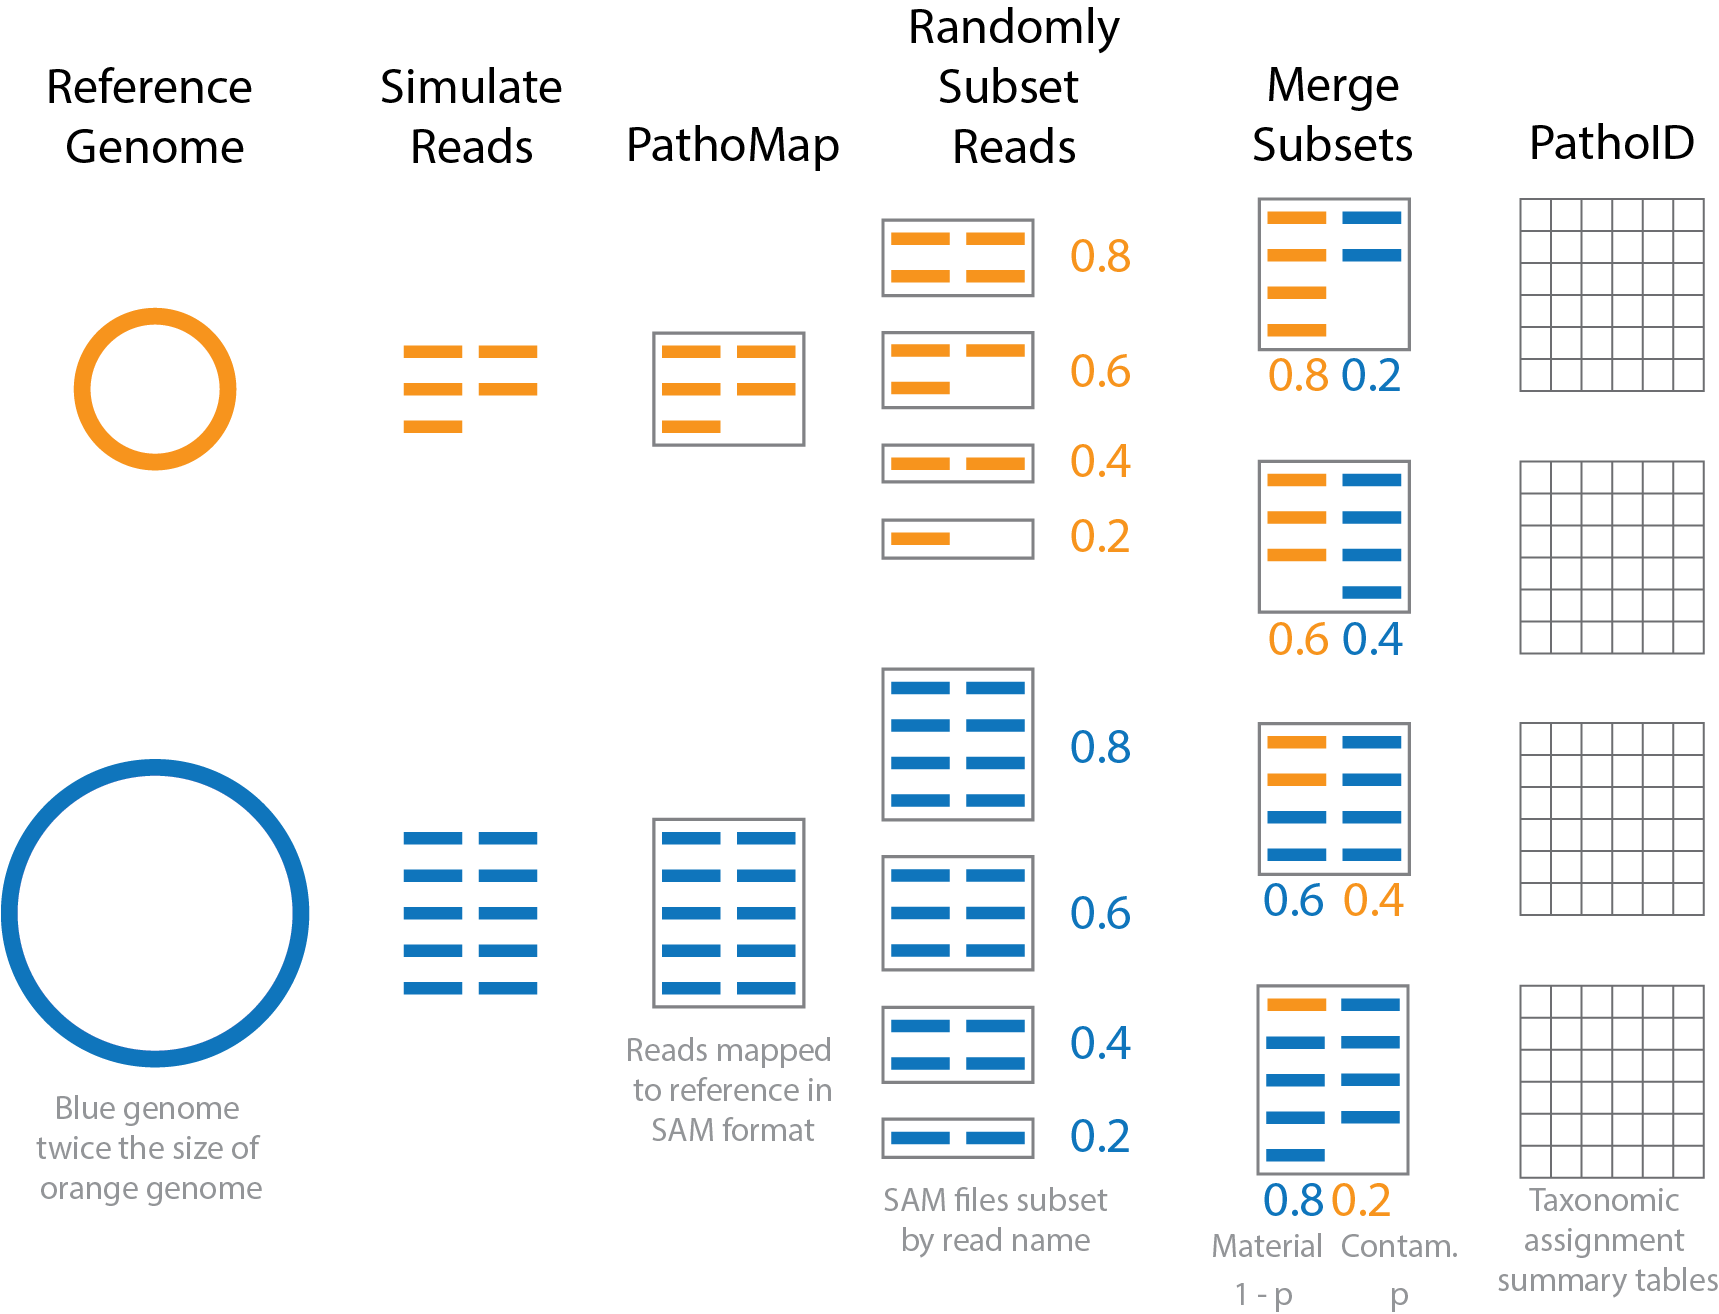
\includegraphics[width=\maxwidth]{figure/contam_simulation} \caption[Diagram of the simulated contaminant dataset workflow for two individual genomes]{Diagram of the simulated contaminant dataset workflow for two individual genomes. Contaminant proportions 0.2 and 0.4 are used for demonstration purposes. The reads were initially simulated from individual genomes. The blue genome is twice the size of the orange genome and twice as many reads are simulated for the blue genome compared to the orange in order to obtain the same coverage. The simulated reads were aligned to the reference database using PathoMap. The resulting alignment file, in SAM file format, was randomly subset based on the desired proportions. Complementary subsets of SAM files (e.g. 0.2 contaminant and 0.8 material) from the two genomes were merged to create individual simulated contaminant datasets.  Due to the different sized genomes, the simulated contaminant datasets have different numbers of reads. Taxonomic assignment summary tables were generated from simulated contaminant datasets using PathoID.}\label{fig:contam_simulation}
\end{figure}


\end{knitrout}


Simulated contaminated datasets were used to evaluate how contaminant detection varied by material and contaminant genome over a range of contaminant concentrations.
Representative genomes for 9 of the 10 genera were used to generate the simulated contaminant datasets (Table \ref{tab:contam_table}).
An \textit{Escherichia coli} strain was selected as a representative of both  and \textit{Shigella} as the genus \textit{Shigella} phylogenetically resides within the species \textit{Escherichia coli} \citep{lan2002escherichia}.
For each pairwise combination of representative genomes, the simulated contaminant dataset was comprised of a randomly selected subset of reads from the material and contaminant simulated single genome sequence dataset (Fig. \ref{fig:contam_simulation}).
The simulated datasets were randomly subsampled at defined proportions, with $p$ representing the proportion of reads from the contaminant single genome dataset, and $1-p$ representing the proportion of reads from the material genome simulated dataset.
A range of contaminant proportions at 10-fold increments were simulated with $p$ ranging from $10^{-1}$ to $10^{-8}$, resulting in 512 simulated contaminant datasets.
This approach simulates the proportions of cells in a contaminated material and not the amount of DNA, assuming unbiased DNA extraction. 
This results in organisms with larger genomes having more simulated reads.  


To generate the simulated contaminant datasets single organism simulated datasets were first generated for the 8 representative genomes using the same methods as used in the baseline assessment (Fig. \ref{fig:contam_simulation}).
The resulting simulated sequencing data was first processed using the PathoQC and PathoMap steps in the Pathoscope pipeline.
The output from the PathoMap step (sam file, sequence alignment file \url{https://samtools.github.io/hts-specs/SAMv1.pdf}) for the material and contaminant datasets were subsampled as described above then combined. 
The resulting SAM file was processed by PathoID, the third step in the Pathoscope pipeline.
Subsampling the sam files instead of the simulated sequence files greatly reduces the computational cost of the analysis as the simulated reads were only processed by the first two steps in Pathoscope pipeline once rather than for every simulated contaminant dataset.


\subsection*{Bioinformatic Pipeline}

%% TODO %%
% Better description for how use of Docker and github promotes repeatability.
%% TODO %%

To facilitate repeatability and transparency, a Docker (\url{www.docker.com}) container is available 
with pre-installed pipeline dependencies (\url{www.registry.hub.docker.com/u/natedolson/docker-pathoscope/}). 
The script used to run the simulations are available at \url{https://github.com/nate-d-olson/genomic_purity}.
Additionally, seed numbers for the random number generator were randomly assigned and recorded for each dataset so the simulated datasets used in the study could be regenerated.
Pathoscope results were processed using the statistical programming language R \citep{R}, and intermediate analysis and data summaries were organized using ProjectTemplate \citep{ProjectTemplate} and archived in a GitHub repository (\url{https://github.com/nate-d-olson/genomic_purity_analysis}) along with the source files for this manuscript.

\section*{Results}

\subsection*{Baseline Assessment Using Individual Genomes}

%% TODO %%
%% Address Jaynes comments for this section
%% TODO %%

First we assessed baseline performance of the proposed method for detecting contaminant DNA in microbial materials. 
Our analysis included taxonomic classification results for simulated sequencing data  from 406 genomes, representing 10 different genera (Table \ref{tab:single_org}). 
For 105 out of the 406 genomes, Pathoscope estimated that less than 99\% of the material was the same species as the genome the sequencing data was simulated from (Fig. \ref{fig:species_prop}). 
The estimated proportion of the material identified as the correct species varied by genus. 
None of the \textit{Shigella} genomes and five of the 49 \textit{Staphylococcus} genomes had estimated proportions greater than 0.9 for the correct species. 
87 of the 105 genomes with estimated species level match proportions less than 0.99 come from \textit{Shigella}, \textit{Staphylococcus}, or \textit{Escherichia}. 
Excluding \textit{Shigella}, \textit{Escherichia}, and \textit{Staphylococcus} the median estimated proportion matching at the species level or higher is  0.9996. 
We characterized false positive contaminants detected in genomes from the genera \textit{Shigella}, \textit{Escherichia}, and \textit{Staphylococcus}, as well as genomes of other species, match proportions less than 0.9. 
Two types of false positive contaminants were identified (1) contaminants that were genomically indistinguishable from the material and (2) contaminants due to errors in the reference database.

% latex table generated in R 3.3.2 by xtable 1.8-2 package
% Mon Nov 14 18:50:54 2016
\begin{table}[ht]
\centering
\begin{tabular}{lrl}
  \hline
Genus & N & Genome Size (Mb) \\ 
  \hline
\textit{Bacillus} &  76 & 5.05 (3.07-7.59) \\ 
  \textit{Escherichia} &  62 & 5.11 (3.98-5.86) \\ 
  \textit{Pseudomonas} &  57 & 6.18 (4.17-7.01) \\ 
  \textit{Staphylococcus} &  49 & 2.82 (2.69-3.08) \\ 
  \textit{Salmonella} &  44 & 4.88 (4.46-5.27) \\ 
  \textit{Listeria} &  39 & 2.97 (2.78-3.11) \\ 
  \textit{Clostridium} &  32 & 4.02 (2.55-6.67) \\ 
  \textit{Yersinia} &  19 & 4.73 (4.62-4.94) \\ 
  \textit{Francisella} &  18 & 1.89 (1.85-2.05) \\ 
  \textit{Shigella} &  10 & 4.74 (4.48-5.22) \\ 
   \hline
\end{tabular}
\caption{Breakdown of the number of genomes by genus used to generate single genome simulated datasets. N indicates the number of genomes, and Genome Size is presented as the median and range (minimum to maximum) genome size} 
\label{tab:single_org}
\end{table}


\begin{knitrout}
\definecolor{shadecolor}{rgb}{0.969, 0.969, 0.969}\color{fgcolor}\begin{figure}
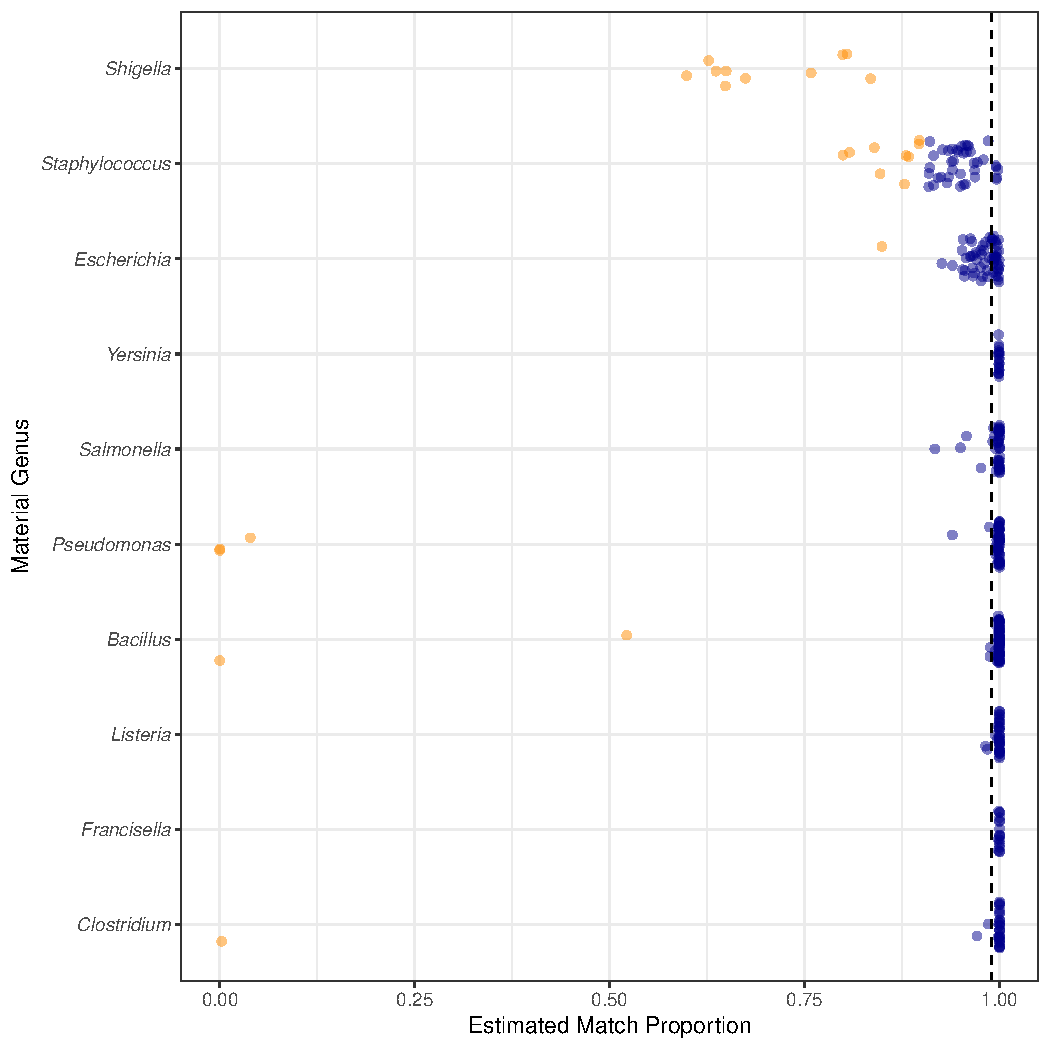
\includegraphics[width=\maxwidth]{figure/species_prop-1} \caption[Species level estimated match proportion varies by material genus]{Species level estimated match proportion varies by material genus. The proportion of the material, simulated sequence data from individual genomes, was estimated by Pathoscope. The estimated match proportion is the total proportion of the material with taxonomic assignments to the genome species, subspecies, strain, or isolate levels. The vertical dashed line indicates the 0.99 match proportion. Orange points are genomes with species level match proportions less than 0.90 and blue points greater than 0.90}\label{fig:species_prop}
\end{figure}


\end{knitrout}

Two genome sequences can be genomically indistinguishable as they are either phylogenetically closely related or share parts of their genome.
Phylogenetic similarity is at least partially responsible for the low species level match proportions for  \textit{Shigella} and \textit{Escherichia}, as \textit{Shigella} is not phylogenetically distinct from \textit{E. coli} \citep{lan2002escherichia}.
When including matches to \textit{E. coli} as species level matches, the median match proportions for \textit{Shigella} genomes increase from 0.66 to 0.92. 
Another example of false positives at the species level due to phylogenetic similarity was low match percentage for \textit{Clostridium autoethanogenum} strain DSM10061 which was due to  \textit{Clostridium ljungdahlii} strain DSM13528 assigned the top proportion (0.998) instead of \textit{C. autoenthanogenum}. 
False positive contaminants due to phylogenetic similarity are not limited to closely related species or genus.
\textit{Escherichia coli} strain UMNK88 low match proportions, was due to two bacteria in the same family as \textit{E. coli} 
(Enterobacteriaceae) \textit{Providencia stuartii} and \textit{Salmonella enterica} subsp. \textit{enterica} serovar Heidelberg with estimated proportions of 0.11 and 0.03 respectively. 

\begin{knitrout}
\definecolor{shadecolor}{rgb}{0.969, 0.969, 0.969}\color{fgcolor}\begin{figure}
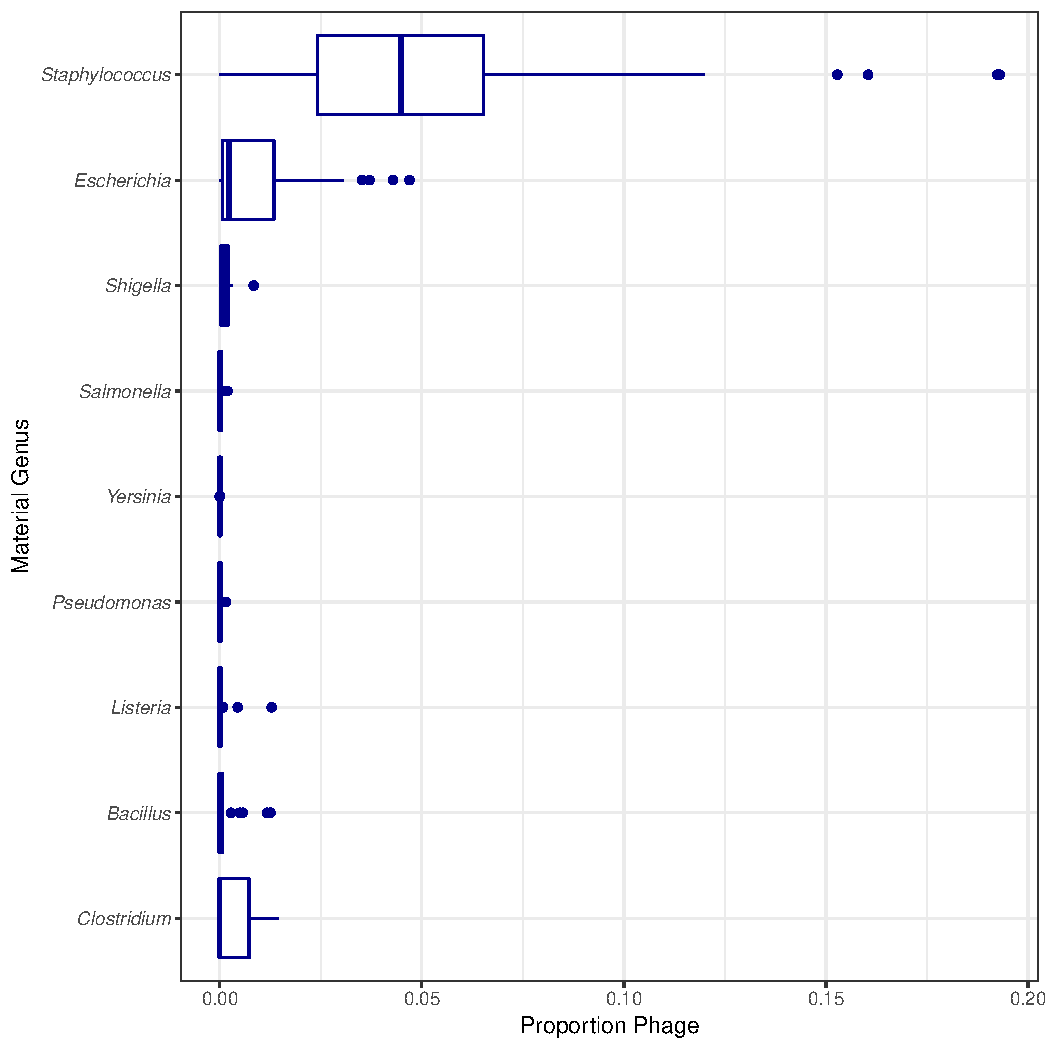
\includegraphics[width=\maxwidth]{figure/phage_prop-1} \caption[Estimated proportion of phage in the simulated single genome datasets by genera]{Estimated proportion of phage in the simulated single genome datasets by genera.  Proportions based on the final estimated proportions for all phage.}\label{fig:phage_prop}
\end{figure}


\end{knitrout}

False positives were also due to sharing of genetic material between organisms. An example of this type of false positive contaminant was phage. 
Phage was identified as false positive contaminants at varying proportions for genomes from all genera investigated, excluding \textit{Francisella} (Fig. \ref{fig:phage_prop}). 
Most notably, the low proportions of species level matches for \textit{E. coli} and \textit{Staphylococcus} are partly due to relatively higher proportions of matches to phage, compared to the other genera investigated. 
Based on phage names all of the false positive phage contaminants were specific to the taxonomy of the genome the sequence data was simulated from. 

False positive contaminants were also due to potential errors in the database such as misclassified or unclassified sequences in the database, genome assemblies in the database including sequence data from organismal or reagent contaminants. 
\textit{Bacillus subtilis} BEST7613 genome had low estimated species level match proportion due to \textit{Synechocystis} sp. PCC 6803 substr. PCC-P being estimated as comprising 47\% of the material  \citep{kanesaki2012identification}. \textit{Synechocystis} is in a different phylum compared to \textit{Bacillus}, cyanobacteria versus firmicutes. 
The high match proportion is potentially due to an error in the database. 
Low species level match proportions can also be due to the database containing unclassified sequence data for organisms highly similar to the material genome. 
For example, the low match proportion for \textit{Pseudomonas} strain FGI182 was due to matches to unclassified bacteria, bacterium 142412, and unclassified \textit{Pseudomonas} species, \textit{Pseudomonas} sp. HF-1. 
The low species proportion of species level matches for \textit{Pseudomonas} strain TKP was also due to misclassified sequences (\textit{Thioalkalivibrio sulfidophilus} strain HL-EbGr7 match proportion 0.0648).

The genome sequences used to populate the reference database can contain contaminants themselves. 
These database contaminants are responsible for additional false positive contaminants.
The eukaryotic false positive contaminants are likely due to contaminants in the material or reagents used to generate the sequencing data used in the assembly \citep{parks2015checkm}. 
The low species proportion of species level matches for \textit{Pseudomonas} strain TKP was partially due to contaminated genome sequences in the database (wheat - \textit{Triticum aestivum} match proportion 0.087). 

\subsection*{Contaminant Detection Assessment}
% latex table generated in R 3.3.2 by xtable 1.8-2 package
% Mon Nov 14 18:50:54 2016
\begin{table}[ht]
\centering
\scalebox{0.65}{
\begin{tabular}{lrllll}
  \hline
Representative Strain & Species & C Mb & C Acc & P Mb & P Acc \\ 
  \hline
Bacillus anthracis str. Ames & 1.00 & 5.23 & AE016879.1 &  &  \\ 
  Clostridium botulinum A str. Hall & 1.00 & 3.76 & CP000727.1 &  &  \\ 
  Escherichia coli O157:H7 str. EC4115 & 0.98 & 5.57 & CP001164.1 & 0.13 & CP001163.1, CP001165.1 \\ 
  Francisella tularensis subsp. tularensis SCHU S4 & 1.00 & 1.89 & AJ749949.2 &  &  \\ 
  Pseudomonas aeruginosa PAO1 & 1.00 & 6.26 & AE004091.2 &  &  \\ 
  Salmonella enterica subsp. enterica serovar Typhimurium str. D23580 & 1.00 & 4.88 & FN424405.1 &  &  \\ 
  Staphylococcus aureus subsp. aureus ED133 & 0.98 & 2.83 & CP001996.1 &  &  \\ 
  Yersinia pestis CO92 & 1.00 & 4.65 & AL590842.1 & 0.18 & AL109969.1, AL117189.1, AL117211.1 \\ 
   \hline
\end{tabular}
}
\caption{Representative strains used in simulated contaminant datasets. When available type strains were selected as the representative genome. Species indicates the proportion of the material assigned to the correct species. DNA size (Mb) and Genbank accession numbers (Acc) are indicated for chromosomes (C) and plasmids (P). Escherichia coli O157:H7 str. EC4115 and Yersinia pestis CO92 have two and three plasmids respectively.} 
\label{tab:contam_table}
\end{table}


%%TODO%% Italicize species names in table caption above

Finally, contaminant detection was assessed using simulated sequencing data from individual genomes. 
Contaminant datasets were developed by combining subsets of simulated data from two organisms at defined proportions,
with the larger proportion representing the microbial material and smaller proportion the contaminant (Fig. \ref{fig:contam_simulation}).
We simulated contaminant datasets as pairwise combinations of representative genomes from 8 of the genera used in the baseline assessment section of the study (Table \ref{tab:contam_table}).
For all of the genomes selected for the detection assessment study, the estimated proportion of material assigned to the correct species was greater than 0.98 (Table \ref{tab:contam_table}).

%%<<contam_min_table, results='asis', echo=FALSE, message=FALSE>>=
%% contam_min_df %>% xtable(label = "tab:contam_min_table", digits=-1, 
%%     caption = "Lowest proportion of contaminant in each pairwise combination of representativ%e genomes detected.") %>%
%%        print(include.rownames=FALSE, scalebox='0.65')
%%@


The minimum contaminant proportion detected was $10 \times 10^{-3}$ and  $10 \times 10^{-4}$ for most pairwise comparisons with a few notable exceptions. 
When \textit{Y. pestis} was the simulated contaminant the minimum detected proportion was 0.1 for all material strains. 
For all simulated datasets where \textit{F. tularensis} was the contaminant the contaminant was not detected.
Conversely, a few contaminants were detected at lower proportions, $10 \times 10^{-8}$, when \textit{Yersinia} was contaminated with \textit{E. coli} as well as when \textit{S. enterica} and \textit{E. coli} contaminated with \textit{B. anthracis}. 
The contaminants detected at lower proportions were false positives in the material single genome simulated datasets. 
For the \textit{E. coli} material dataset with no simulated contaminants, Bacillus sp. SXB had an estimated proportion of \ensuremath{9.2\times 10^{-6}} resulting in an artificially low contaminant detection proportion. 
The simulated contaminant free \texit{Y. pestis} material dataset had two false positives resulting in artifically low contaminant detection proportions Salmonella enterica subsp. enterica serovar Typhi str. CT18 with an estimated proportion of \ensuremath{1.76\times 10^{-5}} and Escherichia coli O104:H4 str. 2011C-3493 with an estimated proportion of \ensuremath{3.77\times 10^{-8}}.

\begin{knitrout}
\definecolor{shadecolor}{rgb}{0.969, 0.969, 0.969}\color{fgcolor}\begin{figure}
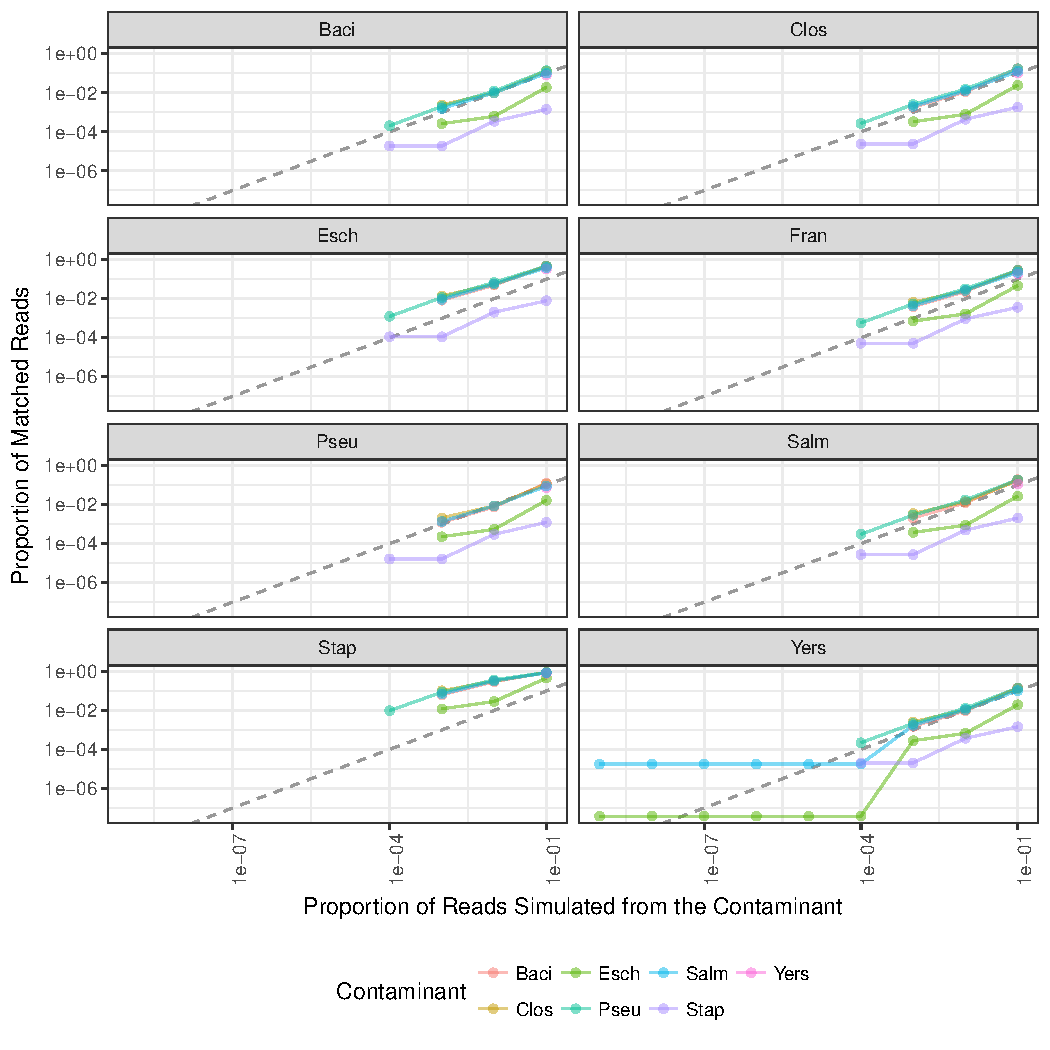
\includegraphics[width=\maxwidth]{figure/contam_fig-1} \caption[Relationship between the proportion of contaminant reads simulated per dataset and the proportion of reads matched to the contaminant genus]{Relationship between the proportion of contaminant reads simulated per dataset and the proportion of reads matched to the contaminant genus. Plots are split by the material genus with line and point color indicating contaminant genus.}\label{fig:contam_fig}
\end{figure}


\end{knitrout}

% <<contam_corr, echo = FALSE, message = FALSE, fig.cap = "Pearson correlation coefficients for estimated and true contaminant proportions.", fig.lp="fig:">>=
% contam_correlation %>% filter(contam_facet != "Yers") %>% 
% ggplot(aes(x = contam_facet, y = target_facet)) + 
%       geom_raster(aes(fill = prop_cor)) + scale_fill_gradient(low = "grey100",high = "grey80") +
%       geom_text(aes(label = round(prop_cor,3))) +
%       theme_bw() + labs(x = "Contaminant", y = "Material")
% @


\begin{knitrout}
\definecolor{shadecolor}{rgb}{0.969, 0.969, 0.969}\color{fgcolor}\begin{figure}
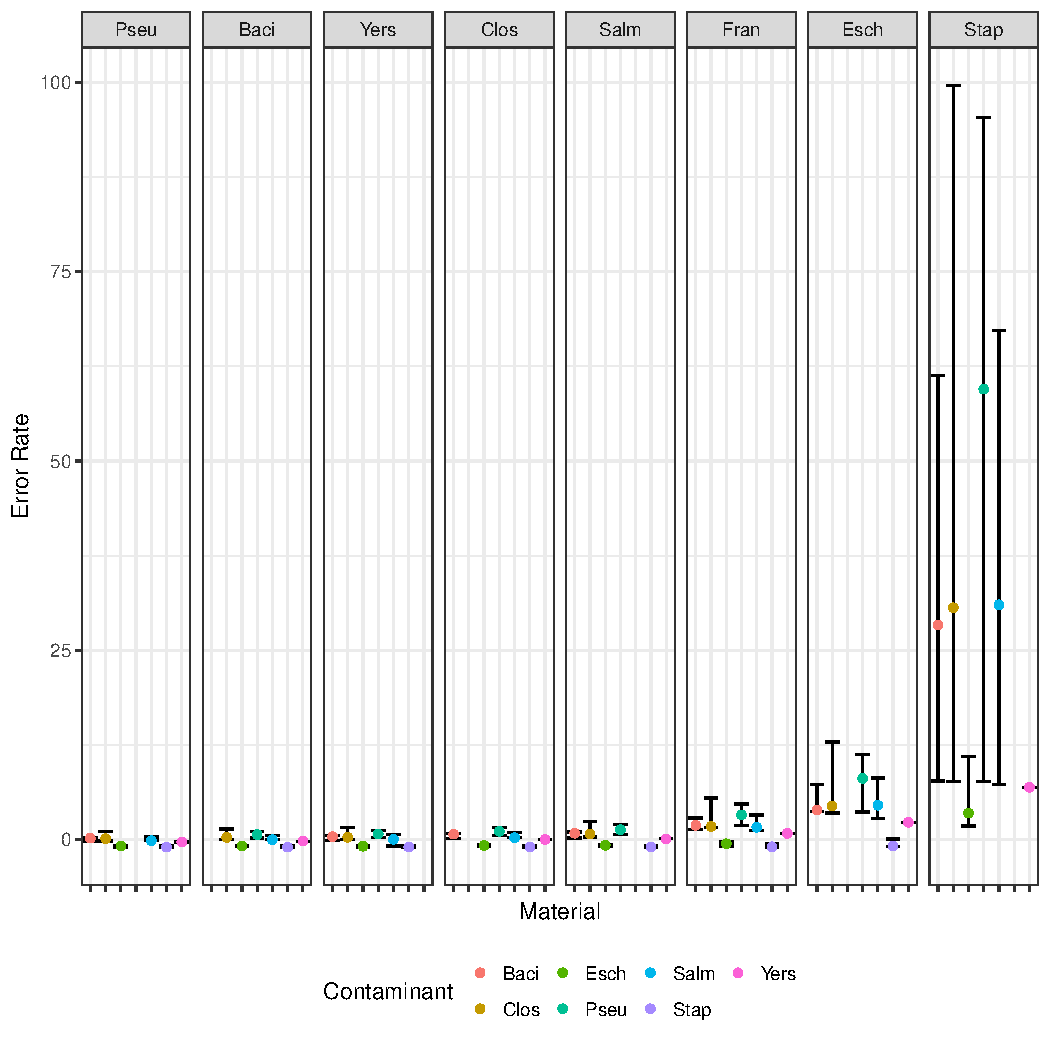
\includegraphics[width=\maxwidth]{figure/contam_resid-1} \caption[Total normalized residuals for pairwise combinations of material and contaminants]{Total normalized residuals for pairwise combinations of material and contaminants.}\label{fig:contam_resid}
\end{figure}


\end{knitrout}


Pearson's correlation coefficient was used to measure the correlation between the estimated contaminant and true contaminant proportions for simulated contaminant proportions greater than $0.1\times 10^{-5}$. 
The estimated and true proportions were strongly correlated for all pairwise comparisons, with an overall median and 95\% confidence interval of 0.99945 (0.96943 - 0.99999) (Fig. \ref{fig:contam_fig}). 
Eight of the pairwise comparisons have correlation coefficients below 0.99, all of which have \textit{S. aureus} as either the contaminant or the material strain. 
Two coefficients were below 0.98, \textit{S. aureus} contaminated with \textit{P. aeruginosa} and \textit{S. enterica}, 0.952 and 0.969 respectively. 
Normalized contaminant proportion residuals, $(estimated-true)/true$, were used to assess the accuracy of the Pathoscope contaminant proportion estimates (Fig. \ref{fig:contam_resid}). 
The material genome strongly influenced the total normalized residuals with \textit{E. coli} and \textit{S. aureus} having consistently higher total normalized residuals compared to the other genomes. 


\section*{Discussion}

The potential for using whole genome sequencing data and taxonomic sequence classification algorithm \textit{Pathoscope} to detect contaminant DNA in microbial materials was evaluated. 
A baseline assessment of the contaminant DNA detection method using simulated sequencing data generated from individual genomes to characterize the types of false positive contaminants identified by the method was performed. 
The false positive contaminants were split into two categories (1) those due to an inability of the method to differentiate the material genome from the contaminant genome and (2) those due to errors in the reference database. 
Variation in contaminant detection was characterized by varying the material, the contaminant, and level of contamination. 
Overall the method was able to identify contaminant proportions at $10 \times 10^{-3}$ for most pairwise contaminant-material combinations. 
However, the accuracy of the estimated proportion of the contaminant in the simulated contaminated material varied by contaminant and material strain. 

A primary limitation of the proposed method is the observed false positive contaminants for single genome simulated sequencing data. 
Performing a baseline assessment of false positive contaminant using simulated sequence data from the microbial material's genome sequence, 
and choosing the appropriate database and taxonomic assignment algorithm can help reduce the impact of false positive on the method's ability to detect contaminant DNA. 
Removing sequences from the database for irrelevant contaminants, such as phage, plasmids, vectors, and multicellular eukaryotes can help reduce the proportion of false positives. 
The relevance of these contaminants is application specific. 
Similarly, using a curated database free of missclassified and unclassified sequence data would further help to reduce the proportion of false positive contaminants \citep{tennessen2015prodege}. 
Pathoscope was used for this proof of concept study as the method uses the full reads and paired-end information for taxonomic classification rather than shorter sequence fragment, $k$-mers. 
Our assumption is that the longer sequence allows for better discrimination between highly similar sequences. 
As there are numerous taxonomic classification algorithms, evaluating multiple methods using sequence data simulated from the material genome of interest can help to determine the optimal comtaminant detection method for a specific microbial material. 
Additionally, false positive contaminants are likely database and taxonomic assignment algorithm dependent. 

%% TODO %% - better dataset read count numbers
Identification and characterization of low abundance contaminants are critical for when the material is used for high sensitivity assays such as PCR. 
The minimum detected contaminant proportion ranged from $10 \times 10^{-3}$ to $10 \times 10^{-4}$ for most simulated contaminant datasets. 
As the individual datasets were simulated at 20X coverage less than 300,000 reads were simulated for each dataset contaminant proportions on average less than 3 reads were spiked into the material datasets for simulated contaminant proportions less than $10 \times 10^{-4}$. 
Unexpectedly low contaminant proportions, $10 \times 10^{-8}$, were detected for \textit{E. coli} contaminanted with \textit{B. anthracis} and \textit{Y. pestis} contaminated with \textit{S. enterica} and \textit{E. coli}. 
The low detection proportions were due to false positive contaminants present in the simulated material single genome dataset used to generate the contaminant mixtures. 
For datasets with \textit{Y. pestis} as the simulated contaminant the minimum detected contaminant proportion was 0.1 and \textit{F. tularensis} was not detected in any simulated contaminant datasets. 
It is unclear why \textit{Y. pestis} was detected at a higher proportion relative to the other datasets, $10 \times 10^{-1}$ versus $10 \times 10^{-3}$, and \textit{F. tularensis} was not detected at all. 
One possible reason for the lower contaminant detect for these two organisms is that there are fewer genomes is the database for these two genera. 
Additionally, the \textit{F. tularensis} dataset is much smaller relative to the other genera, less than 90,000 reads. 
With fewer reads and genomes in the database the probablility that the randomly selected subset of reads spiked into the simulated material dataset contains reads allowing for contaminant detection is lower. 
While the minimum detected contaminant proportion is important for assessing the suitablility of microbial materials for specific applications, quantitative accuracy of the contaminant detection method is important for general material characterization.


The quantitative accuracy of the method varied by material and contaminant, but for all material-contaminant pairs, the Pathoscope estimated and true contaminant proportions were highly correlated. 
While not necessarily relevant to organismal contaminant detection, quantitative accuracy is relevant if the contaminant proportion is included in the material characterization \citep{olson2016pepr}.  
Similar to the false positive contaminant baseline assessment. 
Simulated data can be used to evaluate the minimal detectable contaminant proportion for specific contaminants of interest using different taxonomic assignment algorithms and databases. 
Additionally, sequencing at higher depth theoretically results in lower minimum detectable contaminant proportions and potentially increased quantitative accuracy due to the larger sample size (number of sequences).

\section*{Conclusions}
With the continual decline in the cost of sequencing, advances in sequence analysis methods, whole genome sequencing combined with taxonomic assignment algorithms provides a viable alternative to commonly used organismal contaminant detection methods such as culturing, microscopy, and PCR. 
The method presented here is suitable for detecting organismal contaminants in both genomic DNA and whole cell microbial materials with the only \textit{a priori} assumptions about the contaminant are that it is present in the reference database. 
Furthermore, the method was shown to detect contaminants making up $10 \times 10^{-3}$ proportion of cells in a high-throughput manner. 
Even with the rapid decrease in sequencing cost, whole genome sequencing is more expensive than culture and PCR-based contaminant detection methods. 
However, unlike culture and PCR-based contaminant detection methods, the data generated when whole genome sequencing data is used for organismal contaminant detection can also be used to further characterize the material's genome and potentially identify other characteristics of interest such as the presence of virulence or antibiotic resistance genes. 

\newpage

\section*{Acknowledgments}

The authors would like to thank Dr. Steven Lund for his assistance in developing the study.
The Department of Homeland Security (DHS) Science and Technology Directorate supported this work under the Interagency Agreement HSHQPM-15-T-00019 with the National Institute of Standards and Technology (NIST).
Opinions expressed in this paper are the authors’ and do not necessarily reflect the policies and views of DHS,  NIST, or affiliated venues.
Certain commercial equipment, instruments, or materials are identified in this paper in order to specify the experimental procedure adequately.
Such identification is not intended to imply recommendations or endorsement by NIST,
nor is it intended to imply that the materials or equipment identified are necessarily the best available for the purpose.
Official contribution of NIST; not subject to copyrights in USA.

\bibliography{genomic_purity}

\end{document}
